\section{Role of Smartwatch}

\begin{figure}[b!]
  \centering
    \begin{minipage}{0.20\textwidth}
      \centering
        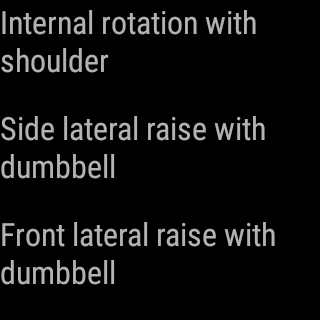
\includegraphics[width=0.80\textwidth]{00_resources/figures/Android_Watch_ListView.png}
    \end{minipage}
    \begin{minipage}{0.20\textwidth}
      \centering
        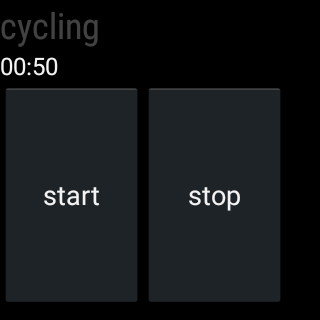
\includegraphics[width=0.80\textwidth]{00_resources/figures/Android_Watch_RecordView.png}
    \end{minipage}
  \caption{Smartwatch user interface}
  \label{fig:smwui}
\end{figure}

The \textit{Android Wear} and \textit{Tizen} smartwatch applications allow the
recording of sensor data to be fed to the algorithm used within the
smartphone application. As shown in figure \ref{fig:smwui}, the user first
selects the exercise to perform after which he or she is presented with the
recording view.

The recording view allows the user to perform the exercise after starting the
recording of sensory data. After the exercise has been performed, the user
manually stops the recording. This allows the smartwatch to send all recorded
data to the smartphone application which in turn feeds the data to the
algorithm. The result is sent back to the smartwatch application and displayed
to the user.

User interfaces of the \textit{Android Wear} and \textit{Tizen} smartwatch
platforms slightly differ due to the nature of the platforms.
